\documentclass[12pt, oneside]{article}   	% use "amsart" instead of "article" for AMSLaTeX format
\usepackage{textcomp}
\usepackage{geometry}                		% See geometry.pdf to learn the layout options. There are lots.
\geometry{letterpaper}                   		% ... or a4paper or a5paper or ...
%\geometry{landscape}                		% Activate for rotated page geometry
%\usepackage[parfill]{parskip}    		% Activate to begin paragraphs with an empty line rather than an indent
\usepackage{graphicx}				% Use pdf, png, jpg, or eps§ with pdflatex; use eps in DVI mode
\usepackage{caption}
\usepackage{subcaption}								% TeX will automatically convert eps --> pdf in pdflatex
\usepackage{color}
\usepackage{amssymb}
\usepackage{amsthm}
\usepackage{url}
\newtheorem{theorem}{Theorem}
\newtheorem{definition}{Definition}
\usepackage{natbib}
\usepackage{xcolor}
% removed hyperref because of arXiv complaining
\usepackage{authblk}
\usepackage{float}
\usepackage{rotating}
\usepackage{adjustbox}
\usepackage[font=small,labelfont=bf]{caption}
%\usepackage{changes}
\usepackage{changes}
\usepackage[colorlinks=false]{hyperref}
\definechangesauthor[name={George Chacko}, color=blue]{gc}

\usepackage{authblk}
\title{Finding Well-Connected Communities in Real-World Networks}
\author[1]{Minhyuk Park\thanks{author order to be determined later}}
\author[1]{Yasamin Tabatabaee\thanks{author order to be determined later}}
\author[1]{Baqiao Liu\thanks{author order to be determined later}}
\author[1]{Placeholder1\thanks{author order to be determined later}}
\author[1]{Placeholder2\thanks{author order to be determined later}}
\author[1]{Placeholder3\thanks{author order to be determined later}}
\author[2]{Dmitriy Korobskiy}
\author[1,3]{George Chacko\thanks{chackoge@illinois.edu}}
\author[1]{Tandy Warnow\thanks{warnow@illinois.edu}}
\affil[1]{Department of Computer Science, University of Illinois Urbana-Champaign, Urbana, IL 61801}
\affil[2]{NTT DATA, McLean, VA 22102}
\affil[3]{Office of Research, Grainger College of Engineering, University of Illinois Urbana-Champaign, Urbana, IL 61801}

% \setlength{\parindent}{0pt}
%SetFonts

% ORCID IDs

% Baqiao Liu: 0000-0002-4210-8269
% Tandy Warnow: 0000-0001-7717-3514
% George Chacko: 0000-0002-2127-1892

\begin{document}
\maketitle

\abstract{Community detection in real-world networks is typically addressed through the use of graph clustering methods that partition the nodes of a
network into disjoint subsets. While  the definition of community varies across methods, it is generally accepted that a elements of a community
should be ``well-connected".  Applying a mild definition of well-connectedness, we explore features of clusters generated by the Leiden algorithm  and the Iterative K-core clustering algorithm. We evaluate
clusters that are produced  by these two approaches for their susceptibility to become disconnected by the deletion of a small number of edges, and find that both methods produce some
clusters that are poorly connected  when applied to real-world networks.  We use a modular pipeline to enable well-connected output clusters, in which allows a user specifies criteria
for a valid  community considering cluster size and minimum edge cut size. We describe the use of this pipeline on real world networks and benchmark networks.
The differences we observe between real world and the synthetic networks are compelling: while clusters produced on real-world networks are often poorly connected, clusters computed
on synthetic networks  generated by the LFR methodology, are more well-connected. A basic assumption of the LFR network generation process  is that every vertex  is in a community; therefore, this  study
suggests the possibility that community structure is not globally found within real-world networks, and that clusterings should be further evaluated.}

\clearpage

\section{Introduction}

The problem of finding communities in complex networks can be posed as a {\em graph partitioning} problem, where the input is a network (a graph with vertices and edges) and the
objective is a partitioning of the vertices into disjoint subsets, so that each of the subsets represents a community \citep{Girvan_2002,Newman_2004}. Community
detection in  large networks has broad applications that include, in scientometrics, the detection of research areas, and author communities \citep{Waltman_2012,Li2014,Fiallos2017,Traag_2019,Chandrasekharan_2020,Wedell2022}.

Disjoint partition is a  common approach to community detection studies \citep{Fortunato2022,Fortunato2010} although variations on this theme arise from different scientific interests \citep{Coscia2011,Schaub2017}.
A common feature of these different formulations is that  the elements of a community are more connected to each other than to those outside the community. In other words, a community
should be {\em well-connected}. Using graph-theoretic terminology, a cluster is said to be well-connected if it does not have a small edge cut, which means that there should not be a small set of edges whose deletion
disconnects the cluster; see discussion in \cite{Traag_2019}.
Note that every edge in  a tree cluster is a cut edge (i.e., a single edge whose removal disconnects the cluster), so that a tree is  a compelling example of a poorly connected cluster.

While the concept of being well-connected depends on the size of the edge cut, the definition of what is ``too small" can be formulated in two
natural ways.
One such  approach, which is used in providing guarantees for the widely used Leiden algorithm \citep{Traag_2019}, specifies the minimum size of an edge cut as a function of the the split  of the cluster into two parts produced
when the edge cut is removed from a cluster.
Specifically, the Leiden guarantee  (Equation D1 in the supplementary informatoin in \cite{Traag_2019}) for an optimal clustering  is that the edge cut size be at least the resolution factor   times he number of possible edges between the two  parts. Writing this formally, and allowing $\gamma$ to be the resolution factor and $E_0$ the edge cut
separating a cluster into two sets $A$ and $B$,  then every edge cut $E_0$ for a cluster in a CPM-optimal clustering is guaranteed to satisfy $$||E_0|| \geq \gamma ||A|| \times ||B||.$$
In other words, this is a {\em lower bound} on the size of an edge cut produced in an optimal CPM-clustering.
Note  that this guarantee is the strongest (meaning the lower bound is largest) when $A$ and $B$ are approximately the same size, and the weakest when the
edge cut separates a single node from the remainder of the cluster.
Note also that this bound depends on the size of the cluster and on   the user-specified value for $\gamma$.
As we show below, the guarantee for CPM-optimal clusters may be very weak for small to moderate clusters, especially for those that are close to being
stars; it will even permit relatively large star-clusters (i.e., clusters containing a single node that is adjacent to all the remaining nodes).

Since the definition for well-connected provided in \cite{Traag_2019} is mainly relevant to large clusters, we consider the
following alternative definition.
Specifically, we require that the size of an edge cut  $E_0$ be above some function that depends only on $||C||$.
Under this definition, a cluster would be considered well-connected if every edge cut, independent of the sizes of the
two sets it creates when deleted, is large enough.
As a simple example, we consider the bound  $$||E_0|| \geq  \lfloor \log_{10}(||C||) \rfloor +1,$$
where $||.||$ denotes the number of elements in the given set and
$\lfloor . \rfloor$ is the floor (largest integer at most the size of the given value).
For example, when $||C|| \leq 9$, this bound only enforces that the cluster be connected, when
$10 \leq ||C|| < 100$ it requires that  the cluster not have any cut edges (single edges that disconnect the cluster), etc.
This formulation offers a relatively weak bound for large clusters (i.e., when   $||C||$ is large), but does provide  a stronger constraint on small to moderate-sized clusters than the
first definition.


Thus, the two approaches provide guarantees about clusters being well-connected for different size clusters, with the first approach a stronger
guarantee for large clusters and the second a stronger guarantee for small to moderate-sized clusters.
Understanding the differences in these guarantees is important, and is part of this study.

To explore well connectedness in community detection, we performed a study to evaluate  clusters produced by two different clustering methods:
the Leiden algorithm  \citep{Traag_2019}, and Iterative K-core Clustering (IKC) \citep{,Wedell2022}.
We designed a pipeline to work with both Leiden and IKC that would ensure that all output clusters satisfy two constraints for being valid communities: (1) each cluster meets a minimum user-specified size requirement
and (2) each cluster is well-connected, using the second criterion provided above, i.e., that  every edge cut $E_0$ in a cluster $C$ satisfy $||E_0|| \geq  \lfloor \log_{10}(||C||) \rfloor +1$.


The pipeline takes a Leiden or IKC clustering as input and then modifies the clustering minimally to ensure that all returned clusters meet these two requirements.
To achieve this, it  first removes all clusters that fail to meet the minimum size specified by the user; we study this method using 11 for this minimum size (i.e., we consider any cluster of size at most 10 to be too small to represent a valid community).
Since any cluster that is a tree (i.e., has no cycles) will fail our connectivity requirement when it has 10 or more vertices, we also remove all trees that remain.
After these two preprocessing steps are complete (i.e., the clusters are ``filtered" to remove small clusters and trees), we move to the heart of the algorithm, the ``Connectivity Modifier".

Within the Connectivity Modifier, we repeatedly examine clusters to see if they are well-connected, according to our requirement.
To do this, we use the VieCut \citep{Henzinger2018,Henzinger2019}  software for finding minimum edge cuts in graphs.
If the cluster does not have a small edge cut (i.e., all its edge cuts are at least the minimum size), then the cluster is not modified by the Connectivity Modifier, and is eturned in the output.
Otherwise, the cluster will be processed in a recursive fashion: first we delete the small edge cut, then we recluster the components that are created (using the specified method -- either Leiden or IKC), and
then we recurse on each cluster that is produced.
At the end of this process, every cluster that remains is well-connected, by our definition.

After running the Connectivity Modifier, we have a set of clusters that are all well-connected. However, some of them may be below our minimum size (default: 11).
Hence, we then check the remaining clusters to see if they are too small (at most 10 nodes), and if so we remove them.
The result of this multi-stage process is a set of clusters that are all well-connected and all at least the specified size.
Furthermore, the original clusters are minimally modified to achieve this, and in particular we never modify an input cluster that is sufficiently large
and meets our edge-connectivity requirement.

Using this pipeline, we evaluate clusterings produced by Leiden and IKC for a number of different networks of different types (i.e., citation networks, social networks, and networks based
on Wikipedia).
We find that both clusterings produce clusters that are either very small (at most 10 nodes) or that fail our minimal connectivity requirement.
We also find that Leiden clusterings reduce in node coverage after being run through this pipeline, indicating  potentially that Leiden clusterings may tend to be too inclusive, but
the degree of impact depends on the network being analyzed as well as on the resolution parameter given to Leiden.
One interesting potential finding is that some real world networks may have large subsets of their nodes that do not belong to any valid community,
thus suggesting that the assumption that clustering methods should place all nodes in communities  may be inappropriate in such cases.

In sum, the pipeline we provide enables the user to minimally modify a given Leiden or IKC clustering to ensure that all final clusters are well-connected,
and in turn also explore the degree to which the study network exhibits community structure throughout the node set.
The pipeline is also very flexible, allowing the user to modify the requirements for validity in output clusters (i.e., changing the minimum cluster size and/or modifying the function for the
size requirement for an edge cut).



\section{Materials and Methods}

\subsection{Methods}
The pipeline we describe is modular, and requires the user to specify values for two algorithmic parameters:
\begin{itemize}
\item $B$, the minimum allowed size of any ``valid" vertex community (default $B=11$)
\item $f(n)$, a function that specifies a minimum size of an edge cut in a cluster with $n$ vertices  for the cluster to be ``well-connected" (default: $ \lfloor \log_{10} n \rfloor +1$)
\item The preferred clustering method, selected from Leiden optimizing CPM (with the resolution value $r$ provided), Leiden optimizing modularity, or the Iterative k-core (IKC) method.
\end{itemize}

\noindent
The input to the pipeline is a network $N$ and the algorithmic parameters as specified.
The pipeline then operates in four stages:
\begin{itemize}
\item
Stage 1: A clustering is generated  from the input network $N$,
\item Stage 2: The clustering is filtered  to remove clusters below size $B$  and any trees,
\item Stage 3: The \emph{Connectivity Modifier} (CM) is applied to each cluster that remains, which results in a set of output clusters are well-connected (based on the function $f(n)$ provided by the user and the selected clustering method), and
\item Stage 4: We remove any resultant clusters below size $B$.
\end{itemize}
By design, this pipeline is guaranteed to return a clustering where each cluster is well-connected (according to the function $f(n)$)  and has size at least $B$.

\begin{figure}[H]
\centering
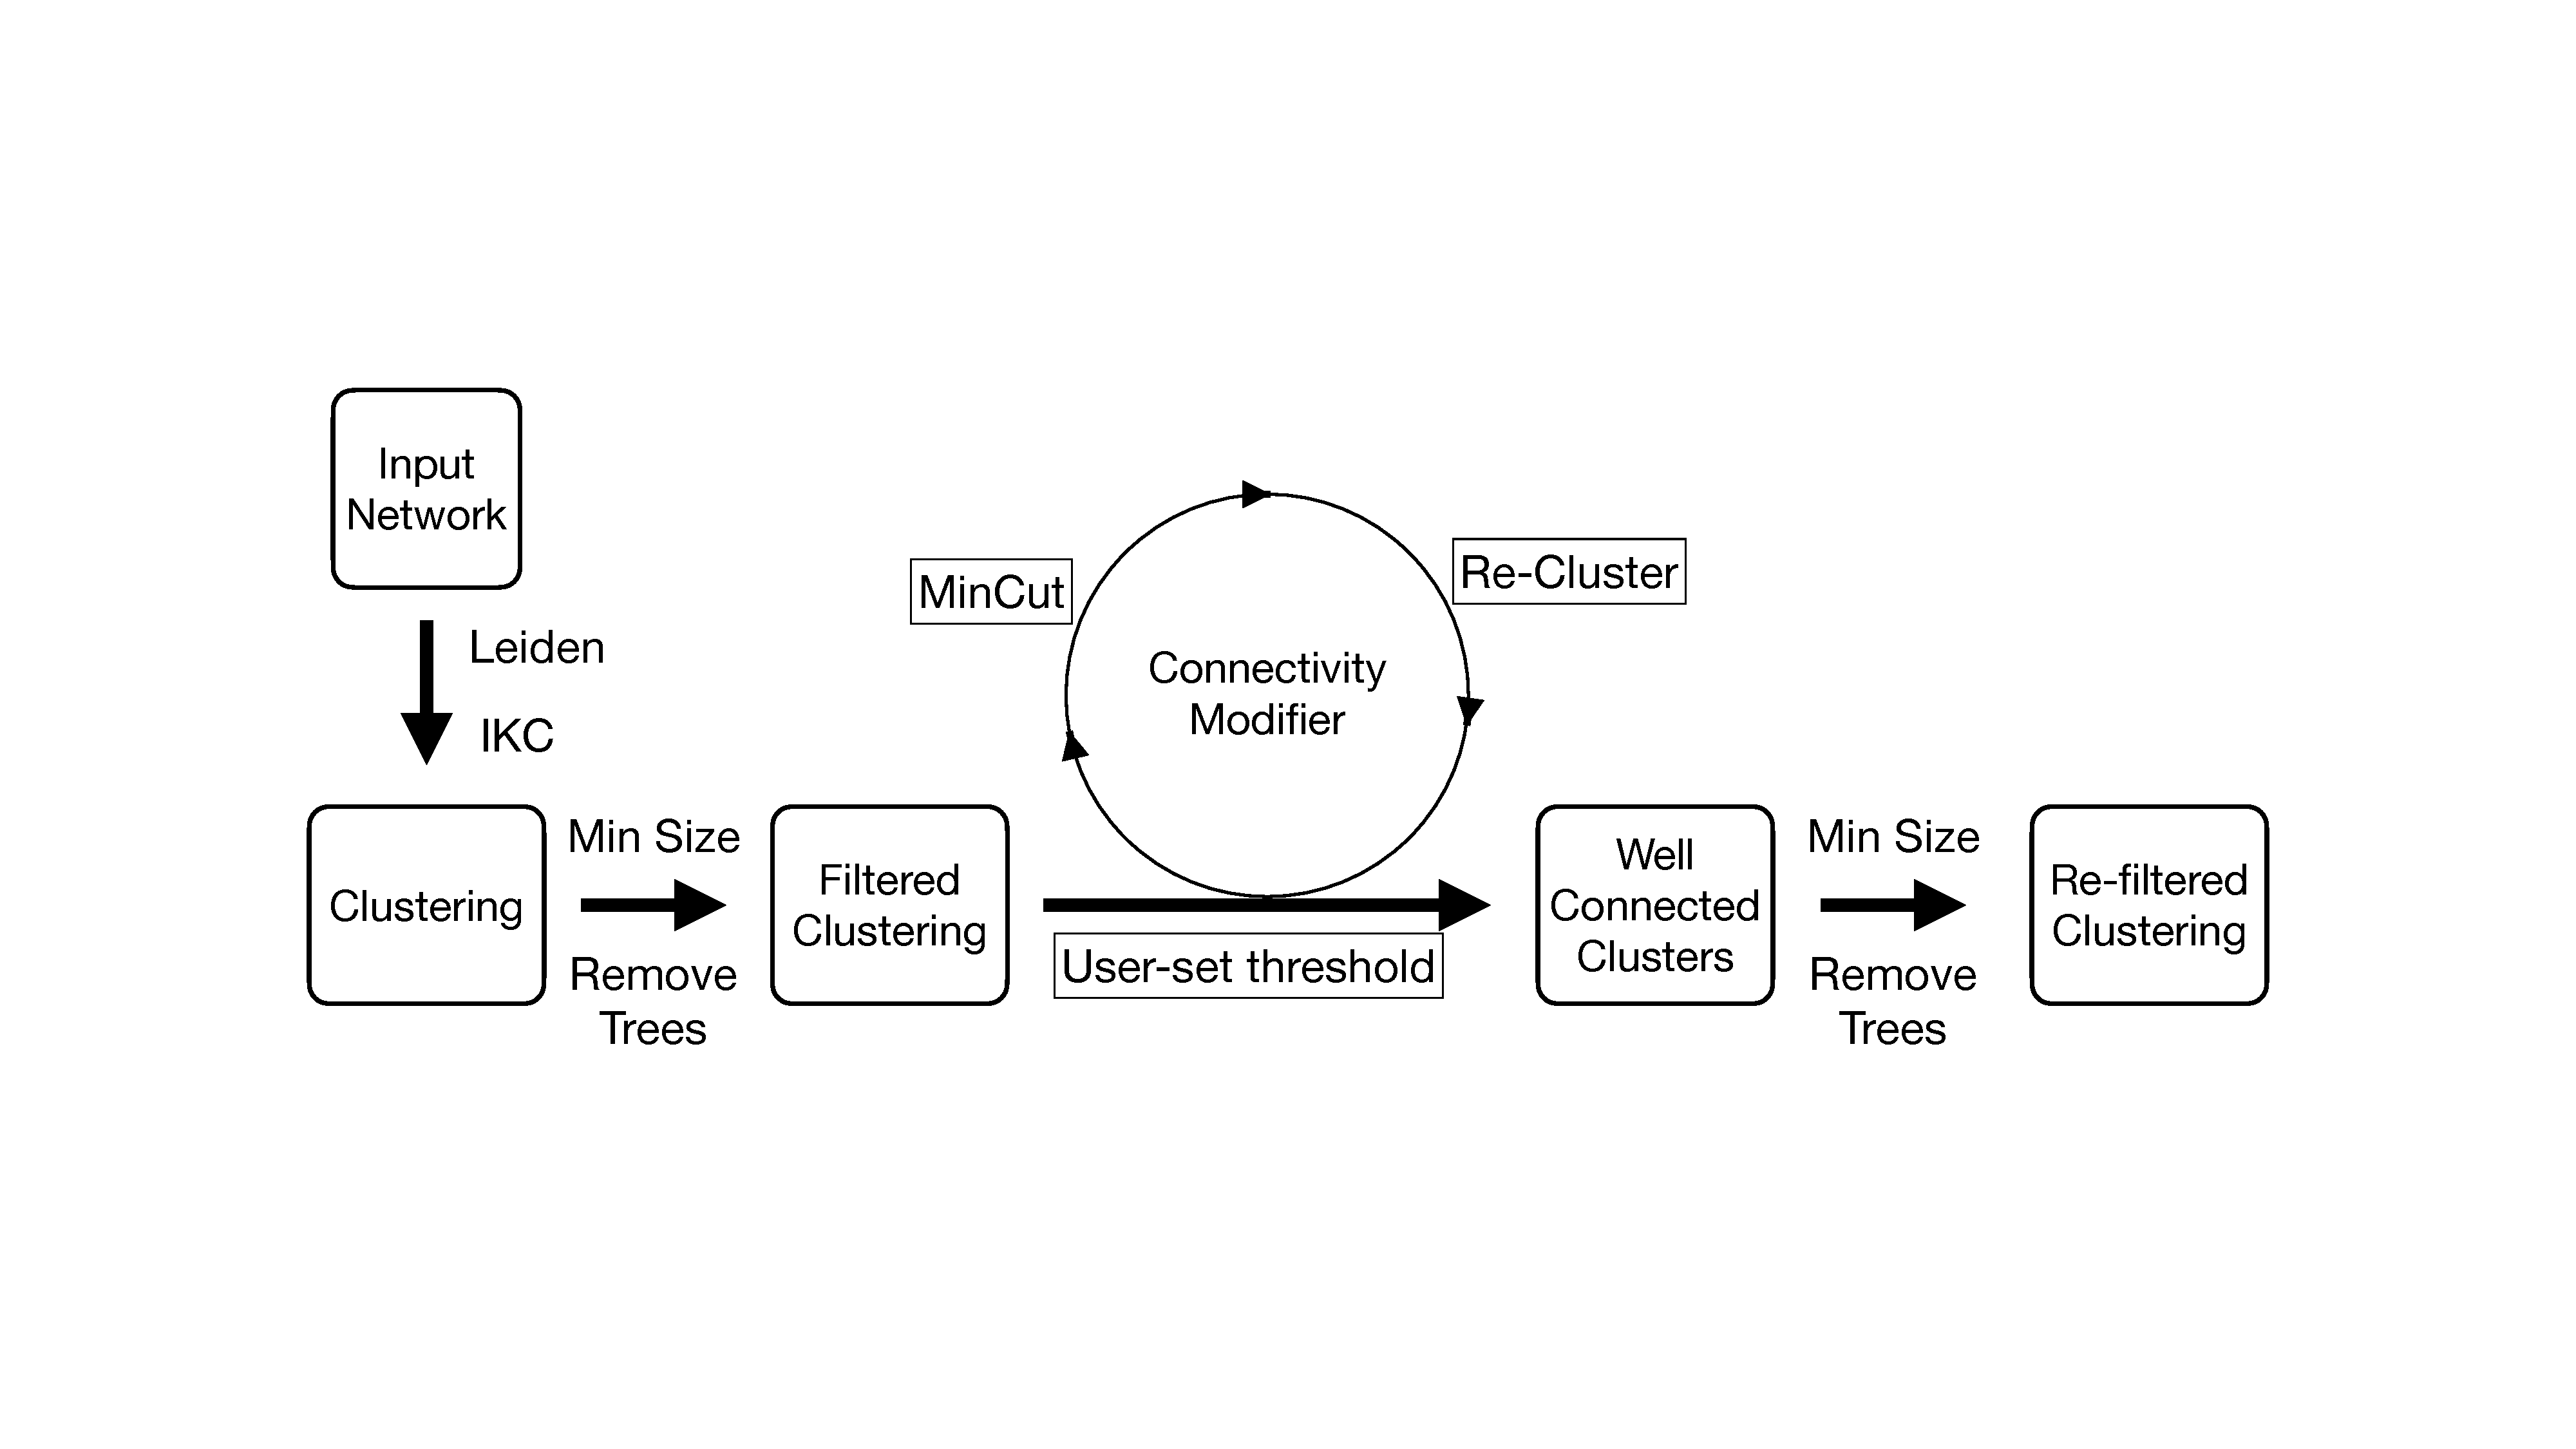
\includegraphics[width=0.7\linewidth]{workflow.pdf}
\caption{Pipeline Schematic. The pipeline depends on user-specified algorithmic parameters (minimum allowed size of a cluster, required minimum number of edges in an edge cut, and clustering method), and operates in four stages:  Stage 1 computes the clustering; Stage 2 removes any clusters that are too small or that are trees;  Stage 3 runs the  Connectivity Modifier to each cluster (i.e., removing small edge cuts if they are below the required size, reclustering, and recursing),  and Stage 4 then removes the clusters that are too small. All clusters that are returned are guaranteed therefore to be well-connected and above the minimum size, both algorithmic parameters specified by the user. }
\end{figure}




In this study, we report results using default values for the algorithmic parameters, which are: $B=11$ (so that all clusters of size at most 10 are considered too small) and requiring that the minimum edge cut for a cluster $C$ be at least  $ 1+ \lfloor \log_{10}(||C||) \rfloor$,  where $||C||$ denotes the number of vertices in $C$.
We report results using both Leiden optimizing CPM with different resolution parameter values and IKC, and we explore results on several networks.


\subsubsection{Filters} Clusters were filtered to remove trees and any cluster of size at most 10, using one of the following tools: (i) a custom R script, (ii) sequential or parallelized Python scripts using the Networkit library \citep{Staudt2016}, or (iii) Belinda, a Python package [cite supplementary information and insert Github reference to https://github.com/illinois-or-research-analytics/belinda] for clustering analysis.

\subsubsection{Connectivity Modifier} To recursively compute and apply minimum cuts to individual clusters, we used the Connectivity Modifier (CM) code at [insert Github reference to Connectivity Modifier], which uses Viecut \citep{Henzinger2018,Henzinger2019} as a dependency, and takes as input a clustering from either the Leiden algorithm or IKC, and returns a set of clusters that is guaranteed to be
well-connected.
We filtered the input clustering as above before passing it as input to Connectivity Modifier. [insert references https://pypi.org/project/connectivity-modifier/].

Here we describe the CM code when passed an input  Leiden clustering $\mathcal{C}$  optimizing CPM (i.e., in default mode). We note that modifying this description to describe how it works with IKC or with Leiden for modularity is straightforward.
We assume that the user has specified the value of the resolution parameter $r$ (referred to as $\gamma$ above and in some publications).
We assume that the minimum size of the edge cut is specified, but recall that our default setting specifies that any edge cut for a cluster $C$ that is at most $ \lfloor \log_{10}(||C||) \rfloor$ is ``too small".
CM used with Leiden and parameter $r$ has the following structure.


First, the set $Bin$ is initialized to the empty set  ($\emptyset$).
CM  then orders the clusters in the input clustering, and   processes each cluster in  turn.
When processing a single cluster $C$,
CM uses VieCut to find a small cut in $C$;  if the cut is too small (i.e., for our default, this means it has at most $\log_{10}(||C||)$ edges), then
we remove the edge cut from the cluster, which splits the cluster $C$ into two  subsets $A$ and $B$.
Both $A$ and $B$ are then reclustered using Leiden with the specified resolution parameter.
Every cluster that results is then recursively analyzed using the same CM pipeline, and the recursion stops when each cluster is considered well-connected.
All the clusters that are produced by this process are therefore well-connected, and are placed in the set $Bin$.

After all clusters are processed, the set $Bin$ is returned.
By design, every cluster in  $Bin$ will be well-connected (i.e., the min cut found using VieCut will be large enough, according to the user-specified criterion).
Furthermore, every cluster in the output will either be one of the input clusters or will be a subset of one of the input clusters.
Finally, every cluster in the input that meets the user-specified criteria for size and edge-connectivity will be found in $Bin$.

\begin{figure}[H]
\centering
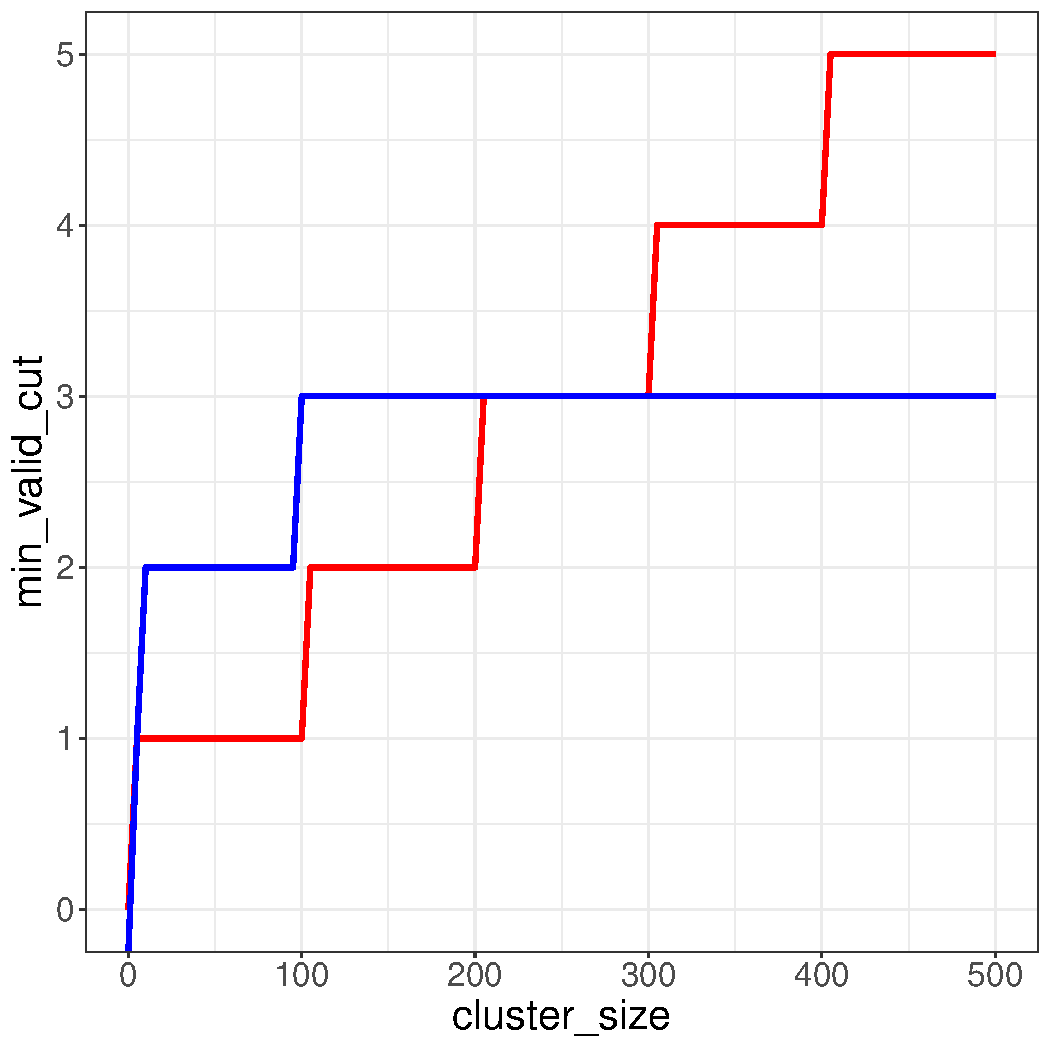
\includegraphics[width=0.7\linewidth]{tandys_figure_3.pdf}
\caption{Comparison of the Leiden definition of well-connected and our definition; each depends on how large the
minimum edge cut can be for the cluster to be considered well-connected.
The bound shown here for Leiden is what is guaranteed for an imbalanced cut of $1$ vertex separated from the remaining $x-1$ vertices
for a cluster with $x$ vertices.
The figure shows two curves: the red one indicates the minimum size for a cut in a well-connected cluster,
according to Leiden Theory (using $r=0.01$) and the blue curve shows the minimum size for a cut in a well-connected cluster according to
our definition.
Accordingly, we see that a cluster with 200 nodes whose minimum cut is of size two, separating one node from the remaining 199 nodes, is considered well-connected
according to Leiden Theory, but not according to our standard of well-connected, which requires that the minimum cut be at least size
3 for any cluster with 200 vertices.  However, once the cluster exceeds size 300, the standard for being well-connected according to
Leiden Theory is stronger than the standard according to our theory. Thus, the two definitions of ``well-connected"  are meaningful in different
regions of cluster size, with Leiden's definition more informative on large clusters (here, above size 301) and our definition more informative on small to moderate-sized clusters (below 201).
The definitions for these minima are: Leiden:  cut size  in a cluster with $x$ vertices must be at least $\lceil r \times (x-1) \rceil$, where $r$ is the resolution parameter (here, $r=0.01$)
and our definition: cut size must be at least $\lfloor(1 + log_{10}x))\rfloor +1$.}
\end{figure}

 \subsection{Data} Several networks were used for testing and analysis and were selected to provide a range of origin, size and edge density. In all cases, below the counts of nodes and edges are reported after removing duplicate records,
self-citations, and parallel edges from the source data.

\paragraph{Curated Exosome Network (CEN)}
The CEN is a citation network focused on the exosome research literature consisting of 13,989,436 nodes and 92,051,051 edges. Its construction has previously been previously described in \cite{Jakatdar_2022}.

\paragraph{Open Citations}
A custom-implemented ETL process was designed to process the publicly available OpenCitations dataset \citep{Peroni2020} and load it into a PostgreSQL table. Citation data was downloaded in Aug 2022. A custom ETL script, written in Bash and SQL, was used to find and pipe uncompressed CSV files, in 20 parallel jobs using the GNU Parallel command-line utility, to a custom function which loaded individual CSV files into a staging view. DOIs were also checked for case differences to remove duplicates.  The resultant network contained 75,025,194 nodes and 1,363,605,603 edges.  [INSERT SECTION ON non-sample based analysis].

\paragraph{SNAP Networks}The following networks were downloaded from the Stanford Network Analysis Project (SNAP) website: (i) cit\_patents \citep{Leskovec2005}, a citation network among US patents (ii) orkut \citep{Yang2013}, data from the Orkut online social network (iii) cit\_hepph \citep{Leskovec2005}, the Arxiv High Energy Physics paper citation network  (iv) wiki\_talk \citep{Leskovec2010}, a network containing users and discussion from the inception of Wikipedia till January 2008 (v) wiki\_topcats \citep{Yin2017}, a web graph of Wikimedia hyperlinks Each network was processed to remove duplicate edges, parallel edges, and self-loops, the numbers of nodes and edges reported below reflect this processing.

\begin{table}[ht]
\centering
\begin{tabular}{rlllr}
  \hline
 & network & edges & nodes & avg\_deg \\
  \hline
  1 & cit\_hepph & 420,877 & 34,546 & 24.37 \\
  2 & cit\_patents & 16,518,947 & 3,774,768 & 8.75 \\
  3 & orkut & 117,185,083 & 3,072,441 & 76.28 \\
  4 & wiki\_talk & 4,659,565 & 2,394,385 & 3.89 \\
  5 & wiki\_topcats & 25,444,207 & 1,791,489 & 28.41 \\
   \hline
\end{tabular}
% Counts manually verified on Jan 31. 2023 by gc
\caption{Network statistics for cleaned versions of 5 networks downloaded from SNAP and used as benchmarks}
\end{table}

\paragraph{LFR (random) networks}
As a comparison group, synthetic networks were generated using the LFR `benchmark' methodology \citep{Lancichinetti2008}. %[Ask Yasamin to write this section up].

We used the LFR benchmark graphs from \cite{lancichinetti2008benchmark} to create simulated networks with ground truth communities, while attempting to emulate the properties of each empirical network and its corresponding Leiden clustering. The generative model of the LFR graphs assume that the node degree and the community size distributions are power-law distributions, a property that is usually seen in large real networks \citep{albert2002statistical}. The software for generating LFR benchmark graphs (available at \href{https://www.santofortunato.net/resources}{https://www.santofortunato.net/resources}) takes the following eight parameters as input:
\begin{itemize}
    \item  \textbf{Node properties:} Number of nodes $N$, average and maximum node degrees ($k$ and $k_{max}$ respectively), and exponent for degree sequence ($\tau_1$) that is assumed to be a power-law.
    \item \textbf{Community properties:} Maximum and minimum community sizes ($c_{max}$ and $c_{min}$), and minus exponent for the community size distribution ($\tau_2$), also modeled as a power-law.
    \item Mixing parameter $\mu$, that is the ratio between the degree of a node outside its community and its total degree, averaged over all nodes in the network. Lower $\mu$ values suggest that the network is constituted from well-separated communities, as nodes are mostly connected to other nodes inside their communities, rather than outside of it.
\end{itemize}


\paragraph{Parameter Estimation.} To emulate real networks using LFR graphs, we estimated all eight parameters described above for a given pair of network $\mathcal{G}$ and a clustering $\mathcal{C}$. Computing $N, k, k_{max}, c_{min}$ and $c_{max}$ is straight-forward using \texttt{networkX} \citep{hagberg2008exploring}. To estimate $\mu$, we do a single iteration over all edges of the network, and for each edge, if the nodes on the two sides of it were in different communities, that edge contribute to the ratio $\mu$ of these two nodes. The total $\mu$ of the network/clustering pair is the average $\mu$ of all nodes.

To estimate $\tau_1$ and $\tau_2$, we fit a power-law distribution to the node degree sequence and the community size distribution, using the approach from \citep{clauset2009power} that is implemented in the \texttt{power-law} Python package \citep{alstott2014powerlaw}. Note that the power-law property may hold for the \textit{tail} of the degree or community size sequence and not the whole distributions. Therefore, following \citep{clauset2009power}, we estimate $x_{min}$, the minimum value for which the power-law property holds as well as the exponent $\alpha$ for the tail of the distribution. Our script for estimating these parameters is available at \href{https://github.com/ytabatabaee/emulate-real-nets}{https://github.com/ytabatabaee/emulate-real-nets}.

\textcolor{blue}{
To do (for Yasamin):}

\begin{itemize}
\item For  the CEN and  for the Open Citations networks, produce one LFR network  that has a mixing parameter and other
parameters set so as to produce something that resembles the given Leiden clustering of the given real-world network. (However, keep the LFR network
on the moderate size, so at most 3,000,000 vertices.)
\textcolor{blue}{This requires that George specify the Leiden clustering for these two networks.}  \textcolor{red}{per discussion on Feb 1, $<=$ 5,000,000 nodes was agreed on).}
\item
For each LFR network:
\begin{itemize}
\item Report empirical statistics of the network
\item Report empirical statistics of the true clustering
\item capture accuracy relative to `ground' truth
\item
Recluster using Leiden (same resolution value) and then run the CM pipeline.
Record all the usual statistics
\item Run CM on the true clustering.
Report all the usual statistics
\end{itemize}
\end{itemize}

\noindent
The usual statistics are things like:
\begin{itemize}
\item Statistics before running the CM pipeline, including distribution of cluster sizes, node and edge coverage
\item Statistics at each stage of the CM pipeline (percentage of clusters that are deleted due to being trees,
then deleted due to being too small, then the percentage of remaining clusters  that have small edge cuts).
But at the end of the pipeline we also remove small clusters.
Also show total node and edge coverage at the end of each stage of the CM pipeline.
\item
In essence we want to know which clusters in the input survive the entire process, which ones are modified.
We'll want their sizes as well, so we can say things like ``20\% of the input clusters above size 100 have small edge cuts" and
``10\% of the input clusters above size 50 are trees".
\end{itemize}

\section{Results and Discussion}

\subsection{Well connected communities from Leiden and IKC clustering.}

We first evaluated a citation network, the CEN (Materials and Methods) consisting of 13,989,436 nodes and 92,051,051 edges, which captures the relatively recent literature relevant to exosomes and extracellular vesicles. We clustered the CEN using Leiden optimizing CPM with resolution values ranging from 0.5 to 0.001 (Table 1). This range of resolution values brackets the resolution values used by us in earlier studies \citep{Wedell2022,Jakatdar_2022}.

% latex table generated in R 4.1.3 by xtable 1.8-4 package
% Mon Jan 30 22:29:28 2023
% generated by singleton corrected script.
\begin{table}[ht]
\centering
\begin{tabular}{rlrrrrrrr}
  \hline
 & clustering & n=1 & n$>$1 & n$>$10 & min & med & max & node\_cov \\
  \hline
1 & leiden 0.5 & 12,701,653 & 433,557 & 8,503 & 11 & 14 & 68 & 0.97 \\
  2 & leiden 0.1 & 8,341,818 & 516,299 & 273,420 & 11 & 11 & 319 & 23.98 \\
  3 & leiden 0.01 & 3,245,556 & 280,518 & 275,641 & 11 & 28 & 3,186 & 76.52 \\
  4 & leiden 0.001 & 2,172,927 & 66,326 & 65,771 & 11 & 98 & 16,481 & 84.45 \\
   \hline
\end{tabular}
\caption{Clustering the Curated Exosome Network (CEN) with Leiden. Node coverage and cluster size increase as resolution values is decreased. The first column (clustering) shows the resolution value passed as a parameter to Leiden. The next three columns show cluster counts for singleton clusters, non-singleton clusters, and clusters of size $>10$. Minimum, median, and max cluster sizes are shown for clusters of size $>10$. The last column indicates node coverage expressed as a percentage; the count of nodes in clusters of size $>10$ relative to the total number of nodes in the network. }
\label{tab: table1}
\end{table}

Predictably, node coverage increased as resolution values was decreased. Of interest, however, was whether trees, which are excellent examples of poorly connected clusters, were being generated. Accordingly, we searched for trees in clusterings generated by either Leiden or IKC. In both cases, we filtered out clusters of size $10$ or less before evaluating clusters for the presence of trees. Strikingly, we observed trees in Leiden clusterings from resolution values of 0.1, 0.01, and 0.001 but not a 0.5. At resolution value of 0.1, 273,420 clusters were generated of which 254,734 (93.2\%) were trees of size 11. At a resolution value of 0.001, 65,771 clusters were generated were found of which 22,750 (34.6\%) were trees (Figure 1 and Table 2). Interestingly, as resolution values were decreased further, the number of trees decreased but the average tree size increased (Figure 1, Table 3).

\begin{figure}[H]
\centering
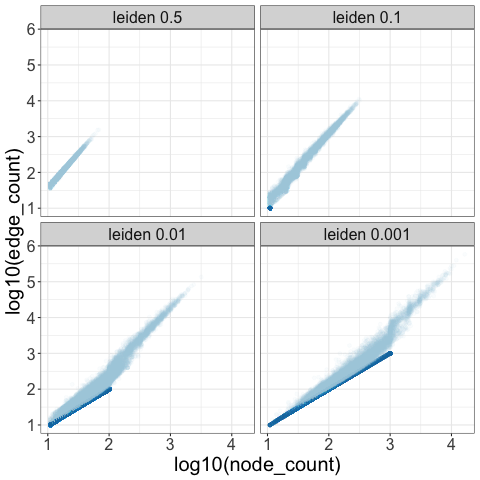
\includegraphics[width=0.7\linewidth]{cen_quad_fig1.png}
\caption{The Curated Exosome Network (CEN) consists of 13,989,436 nodes and 92,051,051 edges. The average degree of its nodes is 13.16. The CEN was clustered at four resolution values (0.5, 0.1, 0.01, 0.001) using the Leiden algorithm with Constant Potts Model as quality function. The figure shows the count of edges in each cluster of size $>$  10 plotted against the count of nodes in each cluster (cluster size). As resolution value decreases, node coverage (the fraction of nodes that are found in clusters of size $>$  10) increases. The number of such clusters does not, however, monotonically increase (Table 1). As the resolution value decreases, tree clusters (dark blue) are detected, with tree size inversely related to resolution value. However, the number of trees decreases as the resolution factor is decreased with the exception of clustering at 0.5 for which no trees are detected. (Table 2).}
\end{figure}

To follow up on the presence of sparse clusters in the form of trees, Leiden clusters were filtered to exclude clusters of size $<=$ 10, after which the number of clusters that were \emph{trees} (the case where \emph{n}, the number of nodes in a cluster, is greater by one than \emph{m}, the number of intra-cluster edges) were counted. Trees were then filtered, after which the remaining clusters were processed with connectivity modifier (CM) using log10(n) as threshold, then filtered again to remove small clusters (Table 2).

% latex table generated in R 4.1.3 by xtable 1.8-4 package
% Sun Jan 29 23:08:57 2023
% generated by running table2.R on odesa in
% /data1/snap_leiden_venv/cen

\begin{table}[ht]
\centering
\begin{tabular}{rllrrrrr}
  \hline
 & clustering & rx & cluster\_count & min & median & max & node\_cov \\
  \hline
1 & leiden.5 & -  & 8503 &  11 & 14.00 &  68 & 0.97 \\
  2 & leiden.5 & filter & 8503 &  11 & 14.00 &  68 & 0.97 \\
  3 & leiden.5 & cm & 8503 &  11 & 14.00 &  68 & 0.97 \\
  4 & leiden.5 & filter & 8503 &  11 & 14.00 &  68 & 0.97 \\
  5 & leiden.1 & - & 273420 &  11 & 11.00 & 319 & 23.98 \\
  6 & leiden.1 & filter & 18686 &  11 & 20.00 & 319 & 3.95 \\
  7 & leiden.1 & cm & 14681 &  11 & 20.00 & 319 & 3.63 \\
  8 & leiden.1 & filter & 14681 &  11 & 20.00 & 319 & 3.63 \\
  9 & leiden.01 & -& 275641 &  11 & 28.00 & 3186 & 76.52 \\
  10 & leiden.01 & filter & 64320 &  11 & 34.00 & 3186 & 24.80 \\
  11 & leiden.01 & cm & 34071 &  11 & 24.00 & 3186 & 13.20 \\
  12 & leiden.01 & filter & 34071 &  11 & 24.00 & 3186 & 13.20 \\
  13 & leiden.001 & - & 65771 &  11 & 98.00 & 16481 & 84.45 \\
  14 & leiden.001 & filter & 43021 &  12 & 112.00 & 16481 & 62.31 \\
  15 & leiden.001 & cm & 27581 &  11 & 32.00 & 16480 & 23.15 \\
  16 & leiden.001 & filter & 27581 &  11 & 32.00 & 16480 & 23.15 \\
   \hline
\end{tabular}
\caption{Identifying well connected clusters from Leiden clustering of the CEN. For each of resolution values \{0.5, 0.1, 0.01, 0.001\}, clusters were limited to those of size 11 or greater, then depleted of trees, the processed by CM, and then filtered to remove any clusters of size 10 or less as well as trees. Node coverage is least 0.5 and maximum at 0.01 (Table 1). However, removal of trees and CM treatment reduces node coverage by 20.4\%, 63.3\%, and 61.3\% of the original values for resolution values of 0.01, 0.01, and 0.001 respectively.  For example, at resolution value 0.001, node coverage drops from 84.45\% to 23.15\%. At a resolution value of 0.5, no change is observed.}
\label{tab:table2}
\end{table}


% latex table generated in R 4.2.2 by xtable 1.8-4 package
% Sun Jan 15 17:37:03 2023
\begin{table}[ht]
\centering
\begin{tabular}{lrllrrr}
  \hline
 Clustering & Resolution & type & min & med & max \\
  \hline
leiden & 0.5 & non\_tree &  11 & 14 &  68 \\
leiden & 0.5 & tree &  NA & NA &  NA \\
leiden & 0.1 & tree &  11 & 11 &  11 \\
leiden  & 0.1 & non\_tree &  11 & 20 & 319 \\
leiden  & 0.01 & tree &  11 & 27 & 101 \\
leiden & 0.01 & non\_tree &  11 & 34 & 3186 \\
leiden & 0.001 & tree &  11 & 65 & 1001 \\
leiden & 0.001 & non\_tree &  12 & 112 & 16481 \\

   \hline
\end{tabular}
\caption{Cluster sizes for Leiden clusters on the CEN. We show empirical statistics (minimum, median, and maximum) of Leiden clusters generated using the Constant Potts Model (CPM) as quality function and with different resolution values. Clusters of of size at most 10 have been removed. Do we need this table?}
\end{table}

% latex table generated in R 4.2.2 by xtable 1.8-4 package
% Fri Jan 13 18:03:02 2023
\begin{table}[ht]
\centering
\begin{tabular}{lrrrrrr}
  \hline
 clustering & res\_value & clus\_count & node\_cov & min & med & max \\
  \hline
Leiden & 0.5 & 297038 & 5.98 &  11 & 13.00 & 183 \\
Leiden & 0.1 & 1313856 & 43.78 &  11 & 17.00 & 882 \\
Leiden & 0.01 & 1361168 & 88.93 &  11 & 19.00 & 3530 \\
Leiden & 0.01 & 232288 & 90.56 &  11 & 64.00 & 23470 \\
Leiden & 0.0005 & 133147 & 90.97 &  11 & 90.00 & 39049 \\
Leiden & 0.0001 & 39069 & 91.81 &  11 & 177.00 & 176557 \\
   \hline
\end{tabular}
\caption{Clustering the Open Citations Network. The open citations network (Materials and Methods) consisting of 75,025,194 nodes and 1,363,605,603 edges was clustered with the Leiden algorithm, using the Constant Potts Model (CPM) as quality function, and using various resolution values (column 1). Node coverage is expressed as the the percent of nodes in these clusters of size $>$ 10 relative to the total number of nodes in the network. Minimum, median, and max cluster sizes are shown in the last three columns.  }
\end{table}

\textcolor{blue}{Insert Minhyuk's IKC data for CEN}.



\section{Conclusions}

\section*{Competing Interests} \vspace{3mm} The authors have no competing interests.

\section*{Funding Information}

\section*{Data Availability}

\section*{Acknowledgments}

\bibliographystyle{apalike}
\bibliography{cmv1}
\end{document}

% latex table generated in R 4.1.3 by xtable 1.8-4 package
% Sun Jan 22 19:56:56 2023
\begin{table}[ht]
\centering
\resizebox{.5\textwidth}{!}{
\begin{tabular}{rrrrrll}
  \hline
 & clus\_count & min & med & max & type & gp \\
  \hline
1 & 20648920 &   2 &   2 &  10 & size 2-10 & leiden.5 \\
  2 & 297038 &  11 &  13 & 183 & size $>$10 & leiden.5 \\
  3 & 297038 &  11 &  13 & 183 & non\_tree & leiden.5 \\
  4 & 10349 &  11 &  13 &  85 & pre-cm & leiden.5 \\
  5 & 10349 &  11 &  13 &  85 & post-cm & leiden.5 \\
  \hline
  6 & 7324830 &   2 &   5 &  10 & size 2-10 & leiden.1 \\
  7 & 1313856 &  11 &  17 & 882 & size $>$10 & leiden.1 \\
  8 & 1299838 &  11 &  17 & 882 & non\_tree & leiden.1 \\
  9 & 14016 &  11 &  11 &  11 & star & leiden.1 \\
  10 &   2 &  11 &  11 &  11 & tree & leiden.1 \\
  11 & 45252 &  11 &  15 & 306 & pre-cm & leiden.1 \\
  12 & 39954 &  11 &  16 & 306 & post-cm & leiden.1 \\
  \hline
  13 & 772769 &   2 &   2 &  10 &  size 2-10 & leiden.01 \\
  14 & 1361168 &  11 &  19 & 3530 & size $>$10 & leiden.01 \\
  15 & 1034558 &  11 &  24 & 3530 & non\_tree & leiden.01 \\
  16 & 8669 &  11 &  18 & 101 & star & leiden.01 \\
  17 & 317941 &  11 &  15 &  58 & tree & leiden.01 \\
  18 & 36171 &  11 &  21 & 1561 & pre-cm & leiden.01 \\
  19 & 29793 &  11 &  16 & 1561 & post-cm & leiden.01 \\
  \hline
  20 & 606966 &   2 &   2 &  10 & size 2-10 & leiden.001 \\
  21 & 232288 &  11 &  64 & 23470 & size $>$10  & leiden.001 \\
  22 & 208543 &  11 &  73 & 23470 & non\_tree & leiden.001 \\
  23 & 1476 &  11 &  15 & 1001 & star & leiden.001 \\
  24 & 22269 &  11 &  43 & 500 & tree & leiden.001 \\
  25 & 7299 &  11 &  63 & 12707 & pre-cm & leiden.001 \\
  26 & 11766 &  11 &  43 & 12707 & post-cm & leiden.001 \\
  \hline
  27 & 522696 &   2 &   2 &  10 & size 2-10 & leiden.0001 \\
  28 & 39069 &  11 & 177 & 176557 & size $>$10 & leiden.0001 \\
  29 & 34031 &  11 & 206 & 176557 & non\_tree & leiden.0001 \\
  30 & 3525 &  11 &  14 & 267 & tree & leiden.0001 \\
  31 & 1513 &  11 &  14 & 251 & star & leiden.0001 \\
  32 & 1192 &  11 & 172 & 53195 & pre-cm & leiden.0001 \\
  33 & 1971 &  11 & 118 & 51053 & post-cm & leiden.0001 \\
   \hline
\end{tabular}}
\caption{test- data being revised to use larger samples}
\end{table}


\paragraph{SNAP benchmarks}
In addition, five more real world networks from the Stanford Network Analysis Project (SNAP) collection \citep{leskovec2016snap} were downloaded in Dec 2022:
\begin{itemize}
\item  \emph{cit\_patents} (3,774,768 nodes, 16,518,947 edges), \
\item \emph{cit\_hepph} (34,546 nodes, 420,877 edges),
\item  \emph{wiki\_topcats} (1,791,489 nodes, 25,444,207 edges)
\item  \emph{orkut} (3,072,441 nodes, 117,185,083 edges).
\item \emph{wiki\_talk} (2,394,385 nodes, 4,659,565 edges)
\end{itemize}
